%%
%% This is file `sample-acmlarge.tex',
%% generated with the docstrip utility.
%%
%% The original source files were:
%%
%% samples.dtx  (with options: `acmlarge')
%% 
%% IMPORTANT NOTICE:
%% 
%% For the copyright see the source file.
%% 
%% Any modified versions of this file must be renamed
%% with new filenames distinct from sample-acmlarge.tex.
%% 
%% For distribution of the original source see the terms
%% for copying and modification in the file samples.dtx.
%% 
%% This generated file may be distributed as long as the
%% original source files, as listed above, are part of the
%% same distribution. (The sources need not necessarily be
%% in the same archive or directory.)
%%
%% The first command in your LaTeX source must be the \documentclass command.
\documentclass[acmlarge,noacm]{acmart}

\settopmatter{printacmref=false} % Removes citation information below abstract
\renewcommand\footnotetextcopyrightpermission[1]{} % removes footnote with conference information in first column
\pagestyle{plain} % removes running headers

%%
%% \BibTeX command to typeset BibTeX logo in the docs
\AtBeginDocument{%
  \providecommand\BibTeX{{%
    \normalfont B\kern-0.5em{\scshape i\kern-0.25em b}\kern-0.8em\TeX}}}

\usepackage{tabu}                      % only used for the table example
\usepackage{booktabs}                  % only used for the table example
\usepackage{multirow}
\usepackage{tabularx}

%%
%% end of the preamble, start of the body of the document source.
\begin{document}

%%
%% The "title" command has an optional parameter,
%% allowing the author to define a "short title" to be used in page headers.
\title{Clustering algorithms on GPU}
\subtitle{Team 18}
%%
%% The "author" command and its associated commands are used to define
%% the authors and their affiliations.
%% Of note is the shared affiliation of the first two authors, and the
%% "authornote" and "authornotemark" commands
%% used to denote shared contribution to the research.
\author{Deepam Sarmah}
\email{deepam20050@iiitd.ac.in}

\renewcommand{\shortauthors}{Deepam Sarmah}

%%
%% This command processes the author and affiliation and title
%% information and builds the first part of the formatted document.
\maketitle

\section{Introduction}
Give an introduction to your project. 100 - 200 words.

\section{Literature review}
Write your literature review of the project topic here. You need to cite relevant papers and online works \cite{roettgervolume}. For example, Strehl and Ghosh \cite{strehl2002cluster} provide an algorithm for combining multiple partitions. These citations will appear in the bibliography section at the end.

\section{Milestones}
Write identified milestones here (at least 4 per team member)

\begin{table}[!h]
\label{tbl:milestones}
\begin{center}
\begin{tabu} to \textwidth {rXl} \toprule
\textbf{S. No.} & \textbf{Milestone} & \textbf{Member}\\\midrule
\multicolumn{3}{c}{\emph{Mid evaluation}}\\
1 & Design GPU data structures for XYZ & Ben Travito\\
2 & Implement min-cut on CPU & Tobin\\
\multicolumn{3}{c}{\emph{Final evaluation}}\\
3 & Implement min-cut on GPU & Travito\\
\bottomrule
\end{tabu}
\end{center}
\end{table}

%\section{Approach}
% Discuss your approach here. (in mid-evaluation submission)
% Include algorithm analysis, challenges and approach.


%\section{Results}
% Discuss results here. (in mid-evaluation submission
% Include output, performance tables and graphs. Comparison with CPU-GPU and with other codes directly related to this work.

% Results may have images.
%\begin{figure}[h]
%  \centering
%  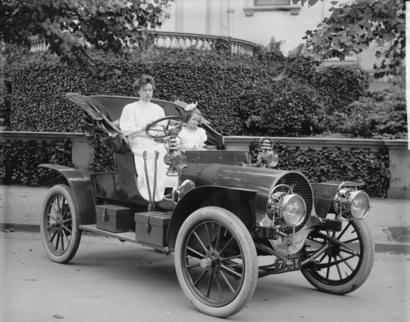
\includegraphics[width=\linewidth]{./images/sample-franklin}
%  \caption{1907 Franklin Model D roadster. Photograph by Harris \&
%    Ewing, Inc. [Public domain], via Wikimedia
%    Commons. (\url{https://goo.gl/VLCRBB}).}
%  \Description{A woman and a girl in white dresses sit in an open car.}
%\end{figure}
%
%Your figures should contain a caption which describes the figure to
%the reader.
%
%Figure captions are placed {\itshape below} the figure.

%\section{Conclusion}
% Conclude here (in final submission)


%%
%% The next two lines define the bibliography style to be used, and
%% the bibliography file.
\bibliographystyle{ACM-Reference-Format}
\bibliography{Report_Project_01_Group_01}

\end{document}